\pgfdeclareplotmark{cross} {
\pgfpathmoveto{\pgfpoint{-0.3\pgfplotmarksize}{\pgfplotmarksize}}
\pgfpathlineto{\pgfpoint{+0.3\pgfplotmarksize}{\pgfplotmarksize}}
\pgfpathlineto{\pgfpoint{+0.3\pgfplotmarksize}{0.3\pgfplotmarksize}}
\pgfpathlineto{\pgfpoint{+1\pgfplotmarksize}{0.3\pgfplotmarksize}}
\pgfpathlineto{\pgfpoint{+1\pgfplotmarksize}{-0.3\pgfplotmarksize}}
\pgfpathlineto{\pgfpoint{+0.3\pgfplotmarksize}{-0.3\pgfplotmarksize}}
\pgfpathlineto{\pgfpoint{+0.3\pgfplotmarksize}{-1.\pgfplotmarksize}}
\pgfpathlineto{\pgfpoint{-0.3\pgfplotmarksize}{-1.\pgfplotmarksize}}
\pgfpathlineto{\pgfpoint{-0.3\pgfplotmarksize}{-0.3\pgfplotmarksize}}
\pgfpathlineto{\pgfpoint{-1.\pgfplotmarksize}{-0.3\pgfplotmarksize}}
\pgfpathlineto{\pgfpoint{-1.\pgfplotmarksize}{0.3\pgfplotmarksize}}
\pgfpathlineto{\pgfpoint{-0.3\pgfplotmarksize}{0.3\pgfplotmarksize}}
\pgfpathclose
\pgfusepathqstroke
}
\pgfdeclareplotmark{cross*} {
\pgfpathmoveto{\pgfpoint{-0.3\pgfplotmarksize}{\pgfplotmarksize}}
\pgfpathlineto{\pgfpoint{+0.3\pgfplotmarksize}{\pgfplotmarksize}}
\pgfpathlineto{\pgfpoint{+0.3\pgfplotmarksize}{0.3\pgfplotmarksize}}
\pgfpathlineto{\pgfpoint{+1\pgfplotmarksize}{0.3\pgfplotmarksize}}
\pgfpathlineto{\pgfpoint{+1\pgfplotmarksize}{-0.3\pgfplotmarksize}}
\pgfpathlineto{\pgfpoint{+0.3\pgfplotmarksize}{-0.3\pgfplotmarksize}}
\pgfpathlineto{\pgfpoint{+0.3\pgfplotmarksize}{-1.\pgfplotmarksize}}
\pgfpathlineto{\pgfpoint{-0.3\pgfplotmarksize}{-1.\pgfplotmarksize}}
\pgfpathlineto{\pgfpoint{-0.3\pgfplotmarksize}{-0.3\pgfplotmarksize}}
\pgfpathlineto{\pgfpoint{-1.\pgfplotmarksize}{-0.3\pgfplotmarksize}}
\pgfpathlineto{\pgfpoint{-1.\pgfplotmarksize}{0.3\pgfplotmarksize}}
\pgfpathlineto{\pgfpoint{-0.3\pgfplotmarksize}{0.3\pgfplotmarksize}}
\pgfpathclose
\pgfusepathqfillstroke
}
\pgfdeclareplotmark{newstar} {
\pgfpathmoveto{\pgfqpoint{0pt}{\pgfplotmarksize}}
\pgfpathlineto{\pgfqpointpolar{44}{0.5\pgfplotmarksize}}
\pgfpathlineto{\pgfqpointpolar{18}{\pgfplotmarksize}}
\pgfpathlineto{\pgfqpointpolar{-20}{0.5\pgfplotmarksize}}
\pgfpathlineto{\pgfqpointpolar{-54}{\pgfplotmarksize}}
\pgfpathlineto{\pgfqpointpolar{-90}{0.5\pgfplotmarksize}}
\pgfpathlineto{\pgfqpointpolar{234}{\pgfplotmarksize}}
\pgfpathlineto{\pgfqpointpolar{198}{0.5\pgfplotmarksize}}
\pgfpathlineto{\pgfqpointpolar{162}{\pgfplotmarksize}}
\pgfpathlineto{\pgfqpointpolar{134}{0.5\pgfplotmarksize}}
\pgfpathclose
\pgfusepathqstroke
}
\pgfdeclareplotmark{newstar*} {
\pgfpathmoveto{\pgfqpoint{0pt}{\pgfplotmarksize}}
\pgfpathlineto{\pgfqpointpolar{44}{0.5\pgfplotmarksize}}
\pgfpathlineto{\pgfqpointpolar{18}{\pgfplotmarksize}}
\pgfpathlineto{\pgfqpointpolar{-20}{0.5\pgfplotmarksize}}
\pgfpathlineto{\pgfqpointpolar{-54}{\pgfplotmarksize}}
\pgfpathlineto{\pgfqpointpolar{-90}{0.5\pgfplotmarksize}}
\pgfpathlineto{\pgfqpointpolar{234}{\pgfplotmarksize}}
\pgfpathlineto{\pgfqpointpolar{198}{0.5\pgfplotmarksize}}
\pgfpathlineto{\pgfqpointpolar{162}{\pgfplotmarksize}}
\pgfpathlineto{\pgfqpointpolar{134}{0.5\pgfplotmarksize}}
\pgfpathclose
\pgfusepathqfillstroke
}
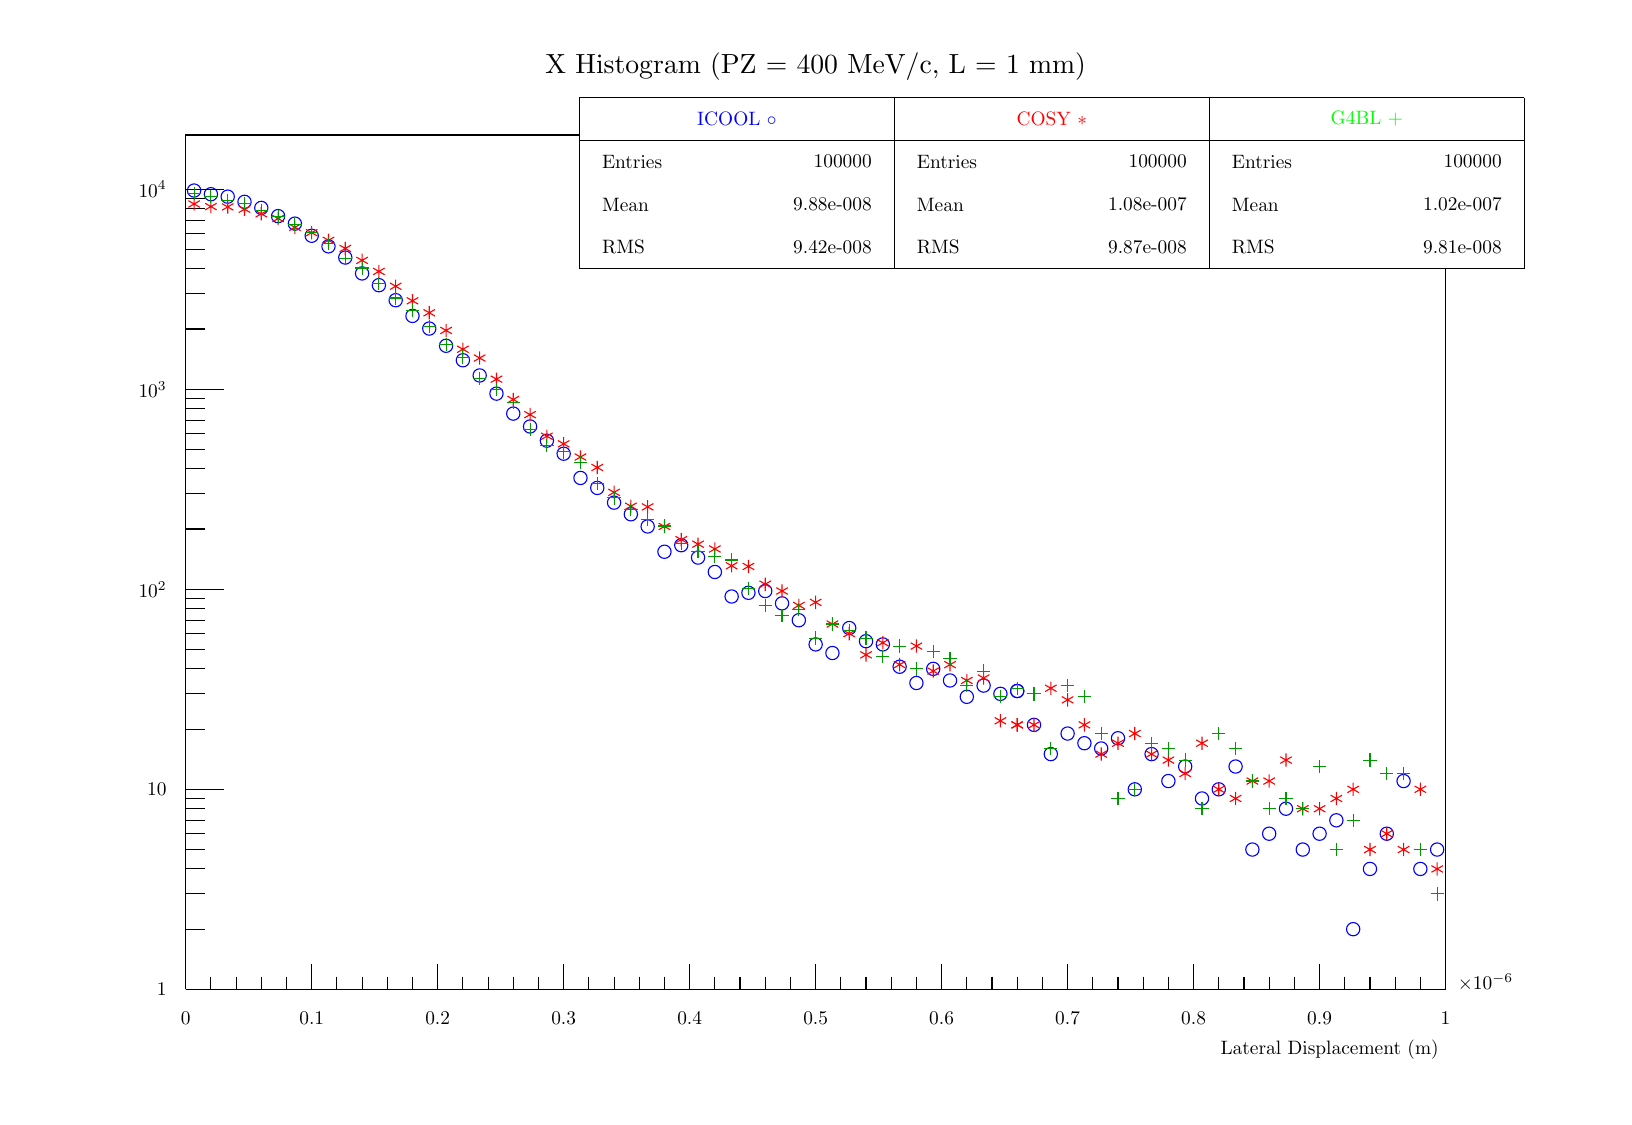
\begin{tikzpicture}
\definecolor{c}{rgb}{1,1,1};
\draw [color=c, fill=c] (0,0) rectangle (20,13.5632);
\draw [color=c, fill=c] (2,1.35632) rectangle (18,12.2069);
\definecolor{c}{rgb}{0,0,0};
\draw [c] (2,1.35632) -- (2,12.2069) -- (18,12.2069) -- (18,1.35632) -- (2,1.35632);
\definecolor{c}{rgb}{1,1,1};
\draw [color=c, fill=c] (2,1.35632) rectangle (18,12.2069);
\definecolor{c}{rgb}{0,0,0};
\draw [c] (2,1.35632) -- (2,12.2069) -- (18,12.2069) -- (18,1.35632) -- (2,1.35632);
\definecolor{c}{rgb}{0,0,1};
\foreach \P in
 {(2.10667,11.5017),(2.32,11.4549),(2.53333,11.4241),(2.74667,11.3581),(2.96,11.2811),(3.17333,11.1766),(3.38667,11.0813),(3.6,10.9273),(3.81333,10.7928),(4.02667,10.6507),(4.24,10.449),(4.45333,10.2999),(4.66667,10.1089),(4.88,9.90959),(5.09333,9.74
886),(5.30667,9.53029),(5.52,9.34637),(5.73333,9.15322),(5.94667,8.92242),(6.16,8.6689),(6.37333,8.50535),(6.58667,8.32531),(6.8,8.15985),(7.01333,7.85163),(7.22667,7.7251),(7.44,7.53825),(7.65333,7.39032),(7.86667,7.23563),(8.08,6.91459),(8.29333,6.
99739),(8.50667,6.8405),(8.72,6.65755),(8.93333,6.34611),(9.14667,6.39307),(9.36,6.41583),(9.57333,6.25878),(9.78667,6.04453),(10,5.73753),(10.2133,5.62819),(10.4267,5.94564),(10.64,5.77841),(10.8533,5.73753),(11.0667,5.45424),(11.28,5.24766),(11.493
3,5.427),(11.7067,5.27964),(11.92,5.07213),(12.1333,5.21471),(12.3467,5.10954),(12.56,5.14572)}{\draw[mark options={color=c,fill=c},mark size=2.402402pt,mark=o] plot coordinates {\P};}
\foreach \P in
 {(12.56,5.14572),(12.7733,4.71595),(12.9867,4.34465),(13.2,4.60551),(13.4133,4.48277),(13.6267,4.41587),(13.84,4.54584),(14.0533,3.89722),(14.2667,4.34465),(14.48,4.0024),(14.6933,4.18674),(14.9067,3.78096),(15.12,3.89722),(15.3333,4.18674),(15.5467
,3.13233),(15.76,3.33353),(15.9733,3.65098),(16.1867,3.13233),(16.4,3.33353),(16.6133,3.50363),(16.8267,2.12121),(17.04,2.8861),(17.2533,3.33353),(17.4667,4.0024),(17.68,2.8861),(17.8933,3.13233)}{\draw[mark options={color=c,fill=c},mark
 size=2.402402pt,mark=o] plot coordinates {\P};}
\definecolor{c}{rgb}{1,1,1};
\draw [color=c, fill=c] (7,10.5115) rectangle (11,12.6816);
\definecolor{c}{rgb}{0,0,0};
\draw [c] (7,10.5115) -- (11,10.5115);
\draw [c] (11,10.5115) -- (11,12.6816);
\draw [c] (11,12.6816) -- (7,12.6816);
\draw [c] (7,12.6816) -- (7,10.5115);
\draw[color=blue](9,12.4103) node[scale=0.7, rotate=0]{ICOOL $\circ$};
\draw [c] (7,12.1391) -- (11,12.1391);
\draw [anchor= west] (7.2,11.8678) node[scale=0.7, rotate=0]{Entries };
\draw [anchor= east] (10.8,11.8678) node[scale=0.7, rotate=0]{ 100000};
\draw [anchor= west] (7.2,11.3253) node[scale=0.7, rotate=0]{Mean  };
\draw [anchor= east] (10.8,11.3253) node[scale=0.7, rotate=0]{ 9.88e-008};
\draw [anchor= west] (7.2,10.7828) node[scale=0.7, rotate=0]{RMS   };
\draw [anchor= east] (10.8,10.7828) node[scale=0.7, rotate=0]{ 9.42e-008};
\draw [c] (2,1.35632) -- (18,1.35632);
\draw [anchor= east] (18,0.596782) node[scale=0.7, rotate=0]{Lateral Displacement (m)};
\draw [c] (2,1.68184) -- (2,1.35632);
\draw [c] (2.32,1.51908) -- (2.32,1.35632);
\draw [c] (2.64,1.51908) -- (2.64,1.35632);
\draw [c] (2.96,1.51908) -- (2.96,1.35632);
\draw [c] (3.28,1.51908) -- (3.28,1.35632);
\draw [c] (3.6,1.68184) -- (3.6,1.35632);
\draw [c] (3.92,1.51908) -- (3.92,1.35632);
\draw [c] (4.24,1.51908) -- (4.24,1.35632);
\draw [c] (4.56,1.51908) -- (4.56,1.35632);
\draw [c] (4.88,1.51908) -- (4.88,1.35632);
\draw [c] (5.2,1.68184) -- (5.2,1.35632);
\draw [c] (5.52,1.51908) -- (5.52,1.35632);
\draw [c] (5.84,1.51908) -- (5.84,1.35632);
\draw [c] (6.16,1.51908) -- (6.16,1.35632);
\draw [c] (6.48,1.51908) -- (6.48,1.35632);
\draw [c] (6.8,1.68184) -- (6.8,1.35632);
\draw [c] (7.12,1.51908) -- (7.12,1.35632);
\draw [c] (7.44,1.51908) -- (7.44,1.35632);
\draw [c] (7.76,1.51908) -- (7.76,1.35632);
\draw [c] (8.08,1.51908) -- (8.08,1.35632);
\draw [c] (8.4,1.68184) -- (8.4,1.35632);
\draw [c] (8.72,1.51908) -- (8.72,1.35632);
\draw [c] (9.04,1.51908) -- (9.04,1.35632);
\draw [c] (9.36,1.51908) -- (9.36,1.35632);
\draw [c] (9.68,1.51908) -- (9.68,1.35632);
\draw [c] (10,1.68184) -- (10,1.35632);
\draw [c] (10.32,1.51908) -- (10.32,1.35632);
\draw [c] (10.64,1.51908) -- (10.64,1.35632);
\draw [c] (10.96,1.51908) -- (10.96,1.35632);
\draw [c] (11.28,1.51908) -- (11.28,1.35632);
\draw [c] (11.6,1.68184) -- (11.6,1.35632);
\draw [c] (11.92,1.51908) -- (11.92,1.35632);
\draw [c] (12.24,1.51908) -- (12.24,1.35632);
\draw [c] (12.56,1.51908) -- (12.56,1.35632);
\draw [c] (12.88,1.51908) -- (12.88,1.35632);
\draw [c] (13.2,1.68184) -- (13.2,1.35632);
\draw [c] (13.52,1.51908) -- (13.52,1.35632);
\draw [c] (13.84,1.51908) -- (13.84,1.35632);
\draw [c] (14.16,1.51908) -- (14.16,1.35632);
\draw [c] (14.48,1.51908) -- (14.48,1.35632);
\draw [c] (14.8,1.68184) -- (14.8,1.35632);
\draw [c] (15.12,1.51908) -- (15.12,1.35632);
\draw [c] (15.44,1.51908) -- (15.44,1.35632);
\draw [c] (15.76,1.51908) -- (15.76,1.35632);
\draw [c] (16.08,1.51908) -- (16.08,1.35632);
\draw [c] (16.4,1.68184) -- (16.4,1.35632);
\draw [c] (16.72,1.51908) -- (16.72,1.35632);
\draw [c] (17.04,1.51908) -- (17.04,1.35632);
\draw [c] (17.36,1.51908) -- (17.36,1.35632);
\draw [c] (17.68,1.51908) -- (17.68,1.35632);
\draw [c] (18,1.68184) -- (18,1.35632);
\draw [c] (18,1.68184) -- (18,1.35632);
\draw [anchor=base] (2,0.908736) node[scale=0.7, rotate=0]{0};
\draw [anchor=base] (3.6,0.908736) node[scale=0.7, rotate=0]{0.1};
\draw [anchor=base] (5.2,0.908736) node[scale=0.7, rotate=0]{0.2};
\draw [anchor=base] (6.8,0.908736) node[scale=0.7, rotate=0]{0.3};
\draw [anchor=base] (8.4,0.908736) node[scale=0.7, rotate=0]{0.4};
\draw [anchor=base] (10,0.908736) node[scale=0.7, rotate=0]{0.5};
\draw [anchor=base] (11.6,0.908736) node[scale=0.7, rotate=0]{0.6};
\draw [anchor=base] (13.2,0.908736) node[scale=0.7, rotate=0]{0.7};
\draw [anchor=base] (14.8,0.908736) node[scale=0.7, rotate=0]{0.8};
\draw [anchor=base] (16.4,0.908736) node[scale=0.7, rotate=0]{0.9};
\draw [anchor=base] (18,0.908736) node[scale=0.7, rotate=0]{1};
\draw [anchor=base west] (18.07,1.35632) node[scale=0.7, rotate=0]{$\times10^{-6}$};
\draw [c] (2,1.35632) -- (2,12.2069);
\draw [c] (2.48,1.35632) -- (2,1.35632);
\draw [anchor= east] (1.844,1.35632) node[scale=0.7, rotate=0]{1};
\draw [c] (2.24,2.12121) -- (2,2.12121);
\draw [c] (2.24,2.56864) -- (2,2.56864);
\draw [c] (2.24,2.8861) -- (2,2.8861);
\draw [c] (2.24,3.13234) -- (2,3.13234);
\draw [c] (2.24,3.33353) -- (2,3.33353);
\draw [c] (2.24,3.50363) -- (2,3.50363);
\draw [c] (2.24,3.65098) -- (2,3.65098);
\draw [c] (2.24,3.78096) -- (2,3.78096);
\draw [c] (2.48,3.89722) -- (2,3.89722);
\draw [anchor= east] (1.844,3.89722) node[scale=0.7, rotate=0]{10};
\draw [c] (2.24,4.66211) -- (2,4.66211);
\draw [c] (2.24,5.10954) -- (2,5.10954);
\draw [c] (2.24,5.427) -- (2,5.427);
\draw [c] (2.24,5.67324) -- (2,5.67324);
\draw [c] (2.24,5.87443) -- (2,5.87443);
\draw [c] (2.24,6.04453) -- (2,6.04453);
\draw [c] (2.24,6.19188) -- (2,6.19188);
\draw [c] (2.24,6.32186) -- (2,6.32186);
\draw [c] (2.48,6.43812) -- (2,6.43812);
\draw [anchor= east] (1.844,6.43812) node[scale=0.7, rotate=0]{$10^{2}$};
\draw [c] (2.24,7.20301) -- (2,7.20301);
\draw [c] (2.24,7.65044) -- (2,7.65044);
\draw [c] (2.24,7.9679) -- (2,7.9679);
\draw [c] (2.24,8.21413) -- (2,8.21413);
\draw [c] (2.24,8.41533) -- (2,8.41533);
\draw [c] (2.24,8.58543) -- (2,8.58543);
\draw [c] (2.24,8.73278) -- (2,8.73278);
\draw [c] (2.24,8.86276) -- (2,8.86276);
\draw [c] (2.48,8.97902) -- (2,8.97902);
\draw [anchor= east] (1.844,8.97902) node[scale=0.7, rotate=0]{$10^{3}$};
\draw [c] (2.24,9.74391) -- (2,9.74391);
\draw [c] (2.24,10.1913) -- (2,10.1913);
\draw [c] (2.24,10.5088) -- (2,10.5088);
\draw [c] (2.24,10.755) -- (2,10.755);
\draw [c] (2.24,10.9562) -- (2,10.9562);
\draw [c] (2.24,11.1263) -- (2,11.1263);
\draw [c] (2.24,11.2737) -- (2,11.2737);
\draw [c] (2.24,11.4037) -- (2,11.4037);
\draw [c] (2.48,11.5199) -- (2,11.5199);
\draw [anchor= east] (1.844,11.5199) node[scale=0.7, rotate=0]{$10^{4}$};
\definecolor{c}{rgb}{1,1,1};
\draw [color=c, fill=c] (7,10.5115) rectangle (11,12.6816);
\definecolor{c}{rgb}{0,0,0};
\draw [c] (7,10.5115) -- (11,10.5115);
\draw [c] (11,10.5115) -- (11,12.6816);
\draw [c] (11,12.6816) -- (7,12.6816);
\draw [c] (7,12.6816) -- (7,10.5115);
\draw[color=blue](9,12.4103) node[scale=0.7, rotate=0]{ICOOL $\circ$};
\draw [c] (7,12.1391) -- (11,12.1391);
\draw [anchor= west] (7.2,11.8678) node[scale=0.7, rotate=0]{Entries };
\draw [anchor= east] (10.8,11.8678) node[scale=0.7, rotate=0]{ 100000};
\draw [anchor= west] (7.2,11.3253) node[scale=0.7, rotate=0]{Mean  };
\draw [anchor= east] (10.8,11.3253) node[scale=0.7, rotate=0]{ 9.88e-008};
\draw [anchor= west] (7.2,10.7828) node[scale=0.7, rotate=0]{RMS   };
\draw [anchor= east] (10.8,10.7828) node[scale=0.7, rotate=0]{ 9.42e-008};
\draw (10,13.0816) node[scale=1, rotate=0]{X Histogram (PZ = 400 MeV/c, L = 1 mm)};
\definecolor{c}{rgb}{1,0,0};
\foreach \P in
 {(2.10667,11.3309),(2.32,11.2981),(2.53333,11.2935),(2.74667,11.264),(2.96,11.2057),(3.17333,11.1459),(3.38667,11.0338),(3.6,10.9663),(3.81333,10.8696),(4.02667,10.7664),(4.24,10.6145),(4.45333,10.474),(4.66667,10.2861),(4.88,10.1013),(5.09333,9.949
23),(5.30667,9.72499),(5.52,9.48588),(5.73333,9.37449),(5.94667,9.10605),(6.16,8.84794),(6.37333,8.65566),(6.58667,8.38171),(6.8,8.28466),(7.01333,8.11731),(7.22667,7.98432),(7.44,7.66868),(7.65333,7.49253),(7.86667,7.484),(8.08,7.23563),(8.29333,7.0
682),(8.50667,7.01061),(8.72,6.94985),(8.93333,6.7361),(9.14667,6.72764),(9.36,6.50242),(9.57333,6.41583),(9.78667,6.23251),(10,6.27169),(10.2133,5.99619),(10.4267,5.87443),(10.64,5.60495),(10.8533,5.75816),(11.0667,5.48083),(11.28,5.71651),(11.4933,
5.39906),(11.7067,5.48083),(11.92,5.27964),(12.1333,5.31073),(12.3467,4.76728),(12.56,4.71595)}{\draw[mark options={color=c,fill=c},mark size=2.402402pt,mark=asterisk] plot coordinates {\P};}
\foreach \P in
 {(12.56,4.71595),(12.7733,4.71595),(12.9867,5.18076),(13.2,5.0334),(13.4133,4.71595),(13.6267,4.34465),(13.84,4.48277),(14.0533,4.60551),(14.2667,4.34465),(14.48,4.26852),(14.6933,4.09841),(14.9067,4.48277),(15.12,3.89722),(15.3333,3.78096),(15.5467
,4.0024),(15.76,4.0024),(15.9733,4.26852),(16.1867,3.65098),(16.4,3.65098),(16.6133,3.78096),(16.8267,3.89722),(17.04,3.13233),(17.2533,3.33353),(17.4667,3.13233),(17.68,3.89722),(17.8933,2.8861)}{\draw[mark options={color=c,fill=c},mark
 size=2.402402pt,mark=asterisk] plot coordinates {\P};}
\definecolor{c}{rgb}{1,1,1};
\draw [color=c, fill=c] (11,10.5115) rectangle (15,12.6816);
\definecolor{c}{rgb}{0,0,0};
\draw [c] (11,10.5115) -- (15,10.5115);
\draw [c] (15,10.5115) -- (15,12.6816);
\draw [c] (15,12.6816) -- (11,12.6816);
\draw [c] (11,12.6816) -- (11,10.5115);
\draw [color=red](13,12.4103) node[scale=0.7, rotate=0]{COSY $*$};
\draw [c] (11,12.1391) -- (15,12.1391);
\draw [anchor= west] (11.2,11.8678) node[scale=0.7, rotate=0]{Entries };
\draw [anchor= east] (14.8,11.8678) node[scale=0.7, rotate=0]{ 100000};
\draw [anchor= west] (11.2,11.3253) node[scale=0.7, rotate=0]{Mean  };
\draw [anchor= east] (14.8,11.3253) node[scale=0.7, rotate=0]{ 1.08e-007};
\draw [anchor= west] (11.2,10.7828) node[scale=0.7, rotate=0]{RMS   };
\draw [anchor= east] (14.8,10.7828) node[scale=0.7, rotate=0]{ 9.87e-008};
\definecolor{c}{rgb}{1,1,1};
\draw [color=c, fill=c] (11,10.5115) rectangle (15,12.6816);
\definecolor{c}{rgb}{0,0,0};
\draw [c] (11,10.5115) -- (15,10.5115);
\draw [c] (15,10.5115) -- (15,12.6816);
\draw [c] (15,12.6816) -- (11,12.6816);
\draw [c] (11,12.6816) -- (11,10.5115);
\draw [color=red](13,12.4103) node[scale=0.7, rotate=0]{COSY $*$};
\draw [c] (11,12.1391) -- (15,12.1391);
\draw [anchor= west] (11.2,11.8678) node[scale=0.7, rotate=0]{Entries };
\draw [anchor= east] (14.8,11.8678) node[scale=0.7, rotate=0]{ 100000};
\draw [anchor= west] (11.2,11.3253) node[scale=0.7, rotate=0]{Mean  };
\draw [anchor= east] (14.8,11.3253) node[scale=0.7, rotate=0]{ 1.08e-007};
\draw [anchor= west] (11.2,10.7828) node[scale=0.7, rotate=0]{RMS   };
\draw [anchor= east] (14.8,10.7828) node[scale=0.7, rotate=0]{ 9.87e-008};
\definecolor{c}{rgb}{0,0.6,0};
\foreach \P in
 {(2.10667,11.4667),(2.32,11.4265),(2.53333,11.3703),(2.74667,11.3347),(2.96,11.2504),(3.17333,11.1695),(3.38667,11.0702),(3.6,10.9705),(3.81333,10.8303),(4.02667,10.6385),(4.24,10.5173),(4.45333,10.318),(4.66667,10.1374),(4.88,9.98351),(5.09333,9.77
492),(5.30667,9.54426),(5.52,9.38675),(5.73333,9.11389),(5.94667,8.97792),(6.16,8.80873),(6.37333,8.46566),(6.58667,8.26587),(6.8,8.18279),(7.01333,8.0477),(7.22667,7.77878),(7.44,7.5977),(7.65333,7.45365),(7.86667,7.32313),(8.08,7.24097),(8.29333,7.
02367),(8.50667,6.92173),(8.72,6.85572),(8.93333,6.80942),(9.14667,6.4491),(9.36,6.23251),(9.57333,6.10585),(9.78667,6.178),(10,5.81782),(10.2133,5.99619),(10.4267,5.91061),(10.64,5.81782),(10.8533,5.58122),(11.0667,5.71651),(11.28,5.427),(11.4933,5.
65094),(11.7067,5.55697),(11.92,5.21471),(12.1333,5.39906),(12.3467,5.07213),(12.56,5.18076)}{\draw[mark options={color=c,fill=c},mark size=2.402402pt,mark=+] plot coordinates {\P};}
\foreach \P in
 {(12.56,5.18076),(12.7733,5.10954),(12.9867,4.41587),(13.2,5.21471),(13.4133,5.07213),(13.6267,4.60551),(13.84,3.78096),(14.0533,3.89722),(14.2667,4.48277),(14.48,4.41587),(14.6933,4.26852),(14.9067,3.65098),(15.12,4.60551),(15.3333,4.41587),(15.546
7,4.0024),(15.76,3.65098),(15.9733,3.78096),(16.1867,3.65098),(16.4,4.18674),(16.6133,3.13233),(16.8267,3.50363),(17.04,4.26852),(17.2533,4.09841),(17.4667,4.09841),(17.68,3.13233),(17.8933,2.56864)}{\draw[mark options={color=c,fill=c},mark
 size=2.402402pt,mark=+] plot coordinates {\P};}
\definecolor{c}{rgb}{1,1,1};
\draw [color=c, fill=c] (15,10.5115) rectangle (19,12.6816);
\definecolor{c}{rgb}{0,0,0};
\draw [c] (15,10.5115) -- (19,10.5115);
\draw [c] (19,10.5115) -- (19,12.6816);
\draw [c] (19,12.6816) -- (15,12.6816);
\draw [c] (15,12.6816) -- (15,10.5115);
\draw [color=green](17,12.4103) node[scale=0.7, rotate=0]{G4BL $+$};
\draw [c] (15,12.1391) -- (19,12.1391);
\draw [anchor= west] (15.2,11.8678) node[scale=0.7, rotate=0]{Entries };
\draw [anchor= east] (18.8,11.8678) node[scale=0.7, rotate=0]{ 100000};
\draw [anchor= west] (15.2,11.3253) node[scale=0.7, rotate=0]{Mean  };
\draw [anchor= east] (18.8,11.3253) node[scale=0.7, rotate=0]{ 1.02e-007};
\draw [anchor= west] (15.2,10.7828) node[scale=0.7, rotate=0]{RMS   };
\draw [anchor= east] (18.8,10.7828) node[scale=0.7, rotate=0]{ 9.81e-008};
\definecolor{c}{rgb}{1,1,1};
\draw [color=c, fill=c] (15,10.5115) rectangle (19,12.6816);
\definecolor{c}{rgb}{0,0,0};
\draw [c] (15,10.5115) -- (19,10.5115);
\draw [c] (19,10.5115) -- (19,12.6816);
\draw [c] (19,12.6816) -- (15,12.6816);
\draw [c] (15,12.6816) -- (15,10.5115);
\draw [color=green](17,12.4103) node[scale=0.7, rotate=0]{G4BL $+$};
\draw [c] (15,12.1391) -- (19,12.1391);
\draw [anchor= west] (15.2,11.8678) node[scale=0.7, rotate=0]{Entries };
\draw [anchor= east] (18.8,11.8678) node[scale=0.7, rotate=0]{ 100000};
\draw [anchor= west] (15.2,11.3253) node[scale=0.7, rotate=0]{Mean  };
\draw [anchor= east] (18.8,11.3253) node[scale=0.7, rotate=0]{ 1.02e-007};
\draw [anchor= west] (15.2,10.7828) node[scale=0.7, rotate=0]{RMS   };
\draw [anchor= east] (18.8,10.7828) node[scale=0.7, rotate=0]{ 9.81e-008};
\end{tikzpicture}
